% Options for packages loaded elsewhere
\PassOptionsToPackage{unicode}{hyperref}
\PassOptionsToPackage{hyphens}{url}
%
\documentclass[
]{article}
\usepackage{amsmath,amssymb}
\usepackage{iftex}
\ifPDFTeX
  \usepackage[T1]{fontenc}
  \usepackage[utf8]{inputenc}
  \usepackage{textcomp} % provide euro and other symbols
\else % if luatex or xetex
  \usepackage{unicode-math} % this also loads fontspec
  \defaultfontfeatures{Scale=MatchLowercase}
  \defaultfontfeatures[\rmfamily]{Ligatures=TeX,Scale=1}
\fi
\usepackage{lmodern}
\ifPDFTeX\else
  % xetex/luatex font selection
\fi
% Use upquote if available, for straight quotes in verbatim environments
\IfFileExists{upquote.sty}{\usepackage{upquote}}{}
\IfFileExists{microtype.sty}{% use microtype if available
  \usepackage[]{microtype}
  \UseMicrotypeSet[protrusion]{basicmath} % disable protrusion for tt fonts
}{}
\makeatletter
\@ifundefined{KOMAClassName}{% if non-KOMA class
  \IfFileExists{parskip.sty}{%
    \usepackage{parskip}
  }{% else
    \setlength{\parindent}{0pt}
    \setlength{\parskip}{6pt plus 2pt minus 1pt}}
}{% if KOMA class
  \KOMAoptions{parskip=half}}
\makeatother
\usepackage{xcolor}
\usepackage[margin=1in]{geometry}
\usepackage{color}
\usepackage{fancyvrb}
\newcommand{\VerbBar}{|}
\newcommand{\VERB}{\Verb[commandchars=\\\{\}]}
\DefineVerbatimEnvironment{Highlighting}{Verbatim}{commandchars=\\\{\}}
% Add ',fontsize=\small' for more characters per line
\usepackage{framed}
\definecolor{shadecolor}{RGB}{248,248,248}
\newenvironment{Shaded}{\begin{snugshade}}{\end{snugshade}}
\newcommand{\AlertTok}[1]{\textcolor[rgb]{0.94,0.16,0.16}{#1}}
\newcommand{\AnnotationTok}[1]{\textcolor[rgb]{0.56,0.35,0.01}{\textbf{\textit{#1}}}}
\newcommand{\AttributeTok}[1]{\textcolor[rgb]{0.13,0.29,0.53}{#1}}
\newcommand{\BaseNTok}[1]{\textcolor[rgb]{0.00,0.00,0.81}{#1}}
\newcommand{\BuiltInTok}[1]{#1}
\newcommand{\CharTok}[1]{\textcolor[rgb]{0.31,0.60,0.02}{#1}}
\newcommand{\CommentTok}[1]{\textcolor[rgb]{0.56,0.35,0.01}{\textit{#1}}}
\newcommand{\CommentVarTok}[1]{\textcolor[rgb]{0.56,0.35,0.01}{\textbf{\textit{#1}}}}
\newcommand{\ConstantTok}[1]{\textcolor[rgb]{0.56,0.35,0.01}{#1}}
\newcommand{\ControlFlowTok}[1]{\textcolor[rgb]{0.13,0.29,0.53}{\textbf{#1}}}
\newcommand{\DataTypeTok}[1]{\textcolor[rgb]{0.13,0.29,0.53}{#1}}
\newcommand{\DecValTok}[1]{\textcolor[rgb]{0.00,0.00,0.81}{#1}}
\newcommand{\DocumentationTok}[1]{\textcolor[rgb]{0.56,0.35,0.01}{\textbf{\textit{#1}}}}
\newcommand{\ErrorTok}[1]{\textcolor[rgb]{0.64,0.00,0.00}{\textbf{#1}}}
\newcommand{\ExtensionTok}[1]{#1}
\newcommand{\FloatTok}[1]{\textcolor[rgb]{0.00,0.00,0.81}{#1}}
\newcommand{\FunctionTok}[1]{\textcolor[rgb]{0.13,0.29,0.53}{\textbf{#1}}}
\newcommand{\ImportTok}[1]{#1}
\newcommand{\InformationTok}[1]{\textcolor[rgb]{0.56,0.35,0.01}{\textbf{\textit{#1}}}}
\newcommand{\KeywordTok}[1]{\textcolor[rgb]{0.13,0.29,0.53}{\textbf{#1}}}
\newcommand{\NormalTok}[1]{#1}
\newcommand{\OperatorTok}[1]{\textcolor[rgb]{0.81,0.36,0.00}{\textbf{#1}}}
\newcommand{\OtherTok}[1]{\textcolor[rgb]{0.56,0.35,0.01}{#1}}
\newcommand{\PreprocessorTok}[1]{\textcolor[rgb]{0.56,0.35,0.01}{\textit{#1}}}
\newcommand{\RegionMarkerTok}[1]{#1}
\newcommand{\SpecialCharTok}[1]{\textcolor[rgb]{0.81,0.36,0.00}{\textbf{#1}}}
\newcommand{\SpecialStringTok}[1]{\textcolor[rgb]{0.31,0.60,0.02}{#1}}
\newcommand{\StringTok}[1]{\textcolor[rgb]{0.31,0.60,0.02}{#1}}
\newcommand{\VariableTok}[1]{\textcolor[rgb]{0.00,0.00,0.00}{#1}}
\newcommand{\VerbatimStringTok}[1]{\textcolor[rgb]{0.31,0.60,0.02}{#1}}
\newcommand{\WarningTok}[1]{\textcolor[rgb]{0.56,0.35,0.01}{\textbf{\textit{#1}}}}
\usepackage{longtable,booktabs,array}
\usepackage{calc} % for calculating minipage widths
% Correct order of tables after \paragraph or \subparagraph
\usepackage{etoolbox}
\makeatletter
\patchcmd\longtable{\par}{\if@noskipsec\mbox{}\fi\par}{}{}
\makeatother
% Allow footnotes in longtable head/foot
\IfFileExists{footnotehyper.sty}{\usepackage{footnotehyper}}{\usepackage{footnote}}
\makesavenoteenv{longtable}
\usepackage{graphicx}
\makeatletter
\def\maxwidth{\ifdim\Gin@nat@width>\linewidth\linewidth\else\Gin@nat@width\fi}
\def\maxheight{\ifdim\Gin@nat@height>\textheight\textheight\else\Gin@nat@height\fi}
\makeatother
% Scale images if necessary, so that they will not overflow the page
% margins by default, and it is still possible to overwrite the defaults
% using explicit options in \includegraphics[width, height, ...]{}
\setkeys{Gin}{width=\maxwidth,height=\maxheight,keepaspectratio}
% Set default figure placement to htbp
\makeatletter
\def\fps@figure{htbp}
\makeatother
\setlength{\emergencystretch}{3em} % prevent overfull lines
\providecommand{\tightlist}{%
  \setlength{\itemsep}{0pt}\setlength{\parskip}{0pt}}
\setcounter{secnumdepth}{-\maxdimen} % remove section numbering
\ifLuaTeX
  \usepackage{selnolig}  % disable illegal ligatures
\fi
\IfFileExists{bookmark.sty}{\usepackage{bookmark}}{\usepackage{hyperref}}
\IfFileExists{xurl.sty}{\usepackage{xurl}}{} % add URL line breaks if available
\urlstyle{same}
\hypersetup{
  pdftitle={Multifactorial Designs: Interactions},
  pdfauthor={Dr Pete McKenna},
  hidelinks,
  pdfcreator={LaTeX via pandoc}}

\title{Multifactorial Designs: Interactions}
\usepackage{etoolbox}
\makeatletter
\providecommand{\subtitle}[1]{% add subtitle to \maketitle
  \apptocmd{\@title}{\par {\large #1 \par}}{}{}
}
\makeatother
\subtitle{C91ED: Advanced Experimental Design}
\author{Dr Pete McKenna}
\date{2025-02-04}

\begin{document}
\maketitle

\hypertarget{chapter-4-interactions}{%
\section{Chapter 4: Interactions}\label{chapter-4-interactions}}

\begin{itemize}
\tightlist
\item
  Important in situations where the effect of one predictor on the
  response depends on the value of another predictor variable. This
  dependency can be interpreted and estimated through the inclusion of
  an interaction term.
\item
  When the relationship between more than one predictor variable is of
  theoretical relevance.
\end{itemize}

\hypertarget{continuous-by-categorical-interactions}{%
\subsubsection{Continuous by categorical
interactions}\label{continuous-by-categorical-interactions}}

\hypertarget{example-context-dwelling-setting-sonic-distraction-and-rt}{%
\paragraph{Example context: Dwelling setting, sonic distraction, and
RT}\label{example-context-dwelling-setting-sonic-distraction-and-rt}}

\begin{itemize}
\tightlist
\item
  examining the effects of sonic distraction on cognitive performance
\item
  ppts assigned to randomly receive different levels of sonic
  distraction (e.g., city sounds, jack-hammer, people yelling etc.)
  while they complete an RT task (e.g., respond quickly as possible to
  flashing light)
\item
  each participant performs the task for a randomly chosen level of
  distraction (0 to 100)
\item
  \(H_{1}\) = urban living makes people's task performance more immune
  to sonic distraction.
\item
  the objective is to compare the relationship between distraction and
  performance for \texttt{city} dwellers vs \texttt{rural} dwellers
\end{itemize}

\textbf{Variables}

\begin{itemize}
\tightlist
\item
  DV = mean RT, with higher levels reflecting slower RTs
\item
  continuous predictor variable, level of sonic distraction
  (\texttt{dist\_level})
\item
  group factor with two levels (\texttt{urban} vs \texttt{rural})
\item
  in this examining sonic distractions, let's assume that the mean RT
  for urban dwellers was 450ms, and that for each unit increase in sonic
  distraction, RT increased by 2:
\end{itemize}

\(Y_{i} = 450 + 2X_{i} + e_{i}\)

\begin{itemize}
\tightlist
\item
  Where mean RT at the intercept (\(\beta_{0}\)) was 450ms
\item
  Each unit increase in RT increased time in the response variable by
  2ms, otherwise known as the slope (\(\beta_{1}\)). So \(X_{i}\) in the
  formula represents the amount of sonic distraction.
\end{itemize}

\hypertarget{simulate-data-for-urban-group}{%
\paragraph{Simulate data for urban
group}\label{simulate-data-for-urban-group}}

\begin{Shaded}
\begin{Highlighting}[]
\FunctionTok{set.seed}\NormalTok{(}\DecValTok{1031}\NormalTok{)}

\NormalTok{n\_subj }\OtherTok{\textless{}{-}}\NormalTok{ 100L  }\CommentTok{\# simulate data for 100 subjects}
\NormalTok{b0\_urban }\OtherTok{\textless{}{-}} \DecValTok{450} \CommentTok{\# y{-}intercept}
\NormalTok{b1\_urban }\OtherTok{\textless{}{-}} \DecValTok{2}   \CommentTok{\# slope}

\CommentTok{\# decomposition table}
\NormalTok{urban }\OtherTok{\textless{}{-}} \FunctionTok{tibble}\NormalTok{(}
  \AttributeTok{subj\_id =} \DecValTok{1}\SpecialCharTok{:}\NormalTok{n\_subj,}
  \AttributeTok{group =} \StringTok{"urban"}\NormalTok{,}
  \AttributeTok{b0 =} \DecValTok{450}\NormalTok{,}
  \AttributeTok{b1 =} \DecValTok{2}\NormalTok{,}
  \AttributeTok{dist\_level =} \FunctionTok{sample}\NormalTok{(}\DecValTok{0}\SpecialCharTok{:}\NormalTok{n\_subj, n\_subj, }\AttributeTok{replace =} \ConstantTok{TRUE}\NormalTok{),}
  \AttributeTok{err =} \FunctionTok{rnorm}\NormalTok{(n\_subj, }\AttributeTok{mean =} \DecValTok{0}\NormalTok{, }\AttributeTok{sd =} \DecValTok{80}\NormalTok{),}
  \AttributeTok{simple\_rt =}\NormalTok{ b0 }\SpecialCharTok{+}\NormalTok{ b1 }\SpecialCharTok{*}\NormalTok{ dist\_level }\SpecialCharTok{+}\NormalTok{ err)}

\NormalTok{urban}
\end{Highlighting}
\end{Shaded}

\begin{verbatim}
## # A tibble: 100 x 7
##    subj_id group    b0    b1 dist_level     err simple_rt
##      <int> <chr> <dbl> <dbl>      <int>   <dbl>     <dbl>
##  1       1 urban   450     2         59  -36.1       532.
##  2       2 urban   450     2         45  128.        668.
##  3       3 urban   450     2         55   23.5       584.
##  4       4 urban   450     2          8    1.04      467.
##  5       5 urban   450     2         47   48.7       593.
##  6       6 urban   450     2         96   88.2       730.
##  7       7 urban   450     2         62  110.        684.
##  8       8 urban   450     2          8  -91.6       374.
##  9       9 urban   450     2         15 -109.        371.
## 10      10 urban   450     2         70   20.7       611.
## # i 90 more rows
\end{verbatim}

\begin{itemize}
\tightlist
\item
  Plot the data with line of best fit
\end{itemize}

\begin{Shaded}
\begin{Highlighting}[]
\FunctionTok{ggplot}\NormalTok{(urban, }\FunctionTok{aes}\NormalTok{(dist\_level, simple\_rt)) }\SpecialCharTok{+} 
  \FunctionTok{geom\_point}\NormalTok{(}\AttributeTok{alpha =}\NormalTok{ .}\DecValTok{2}\NormalTok{) }\SpecialCharTok{+}
  \FunctionTok{geom\_smooth}\NormalTok{(}\AttributeTok{method =} \StringTok{"lm"}\NormalTok{, }\AttributeTok{se =} \ConstantTok{FALSE}\NormalTok{)}
\end{Highlighting}
\end{Shaded}

\begin{verbatim}
## `geom_smooth()` using formula = 'y ~ x'
\end{verbatim}

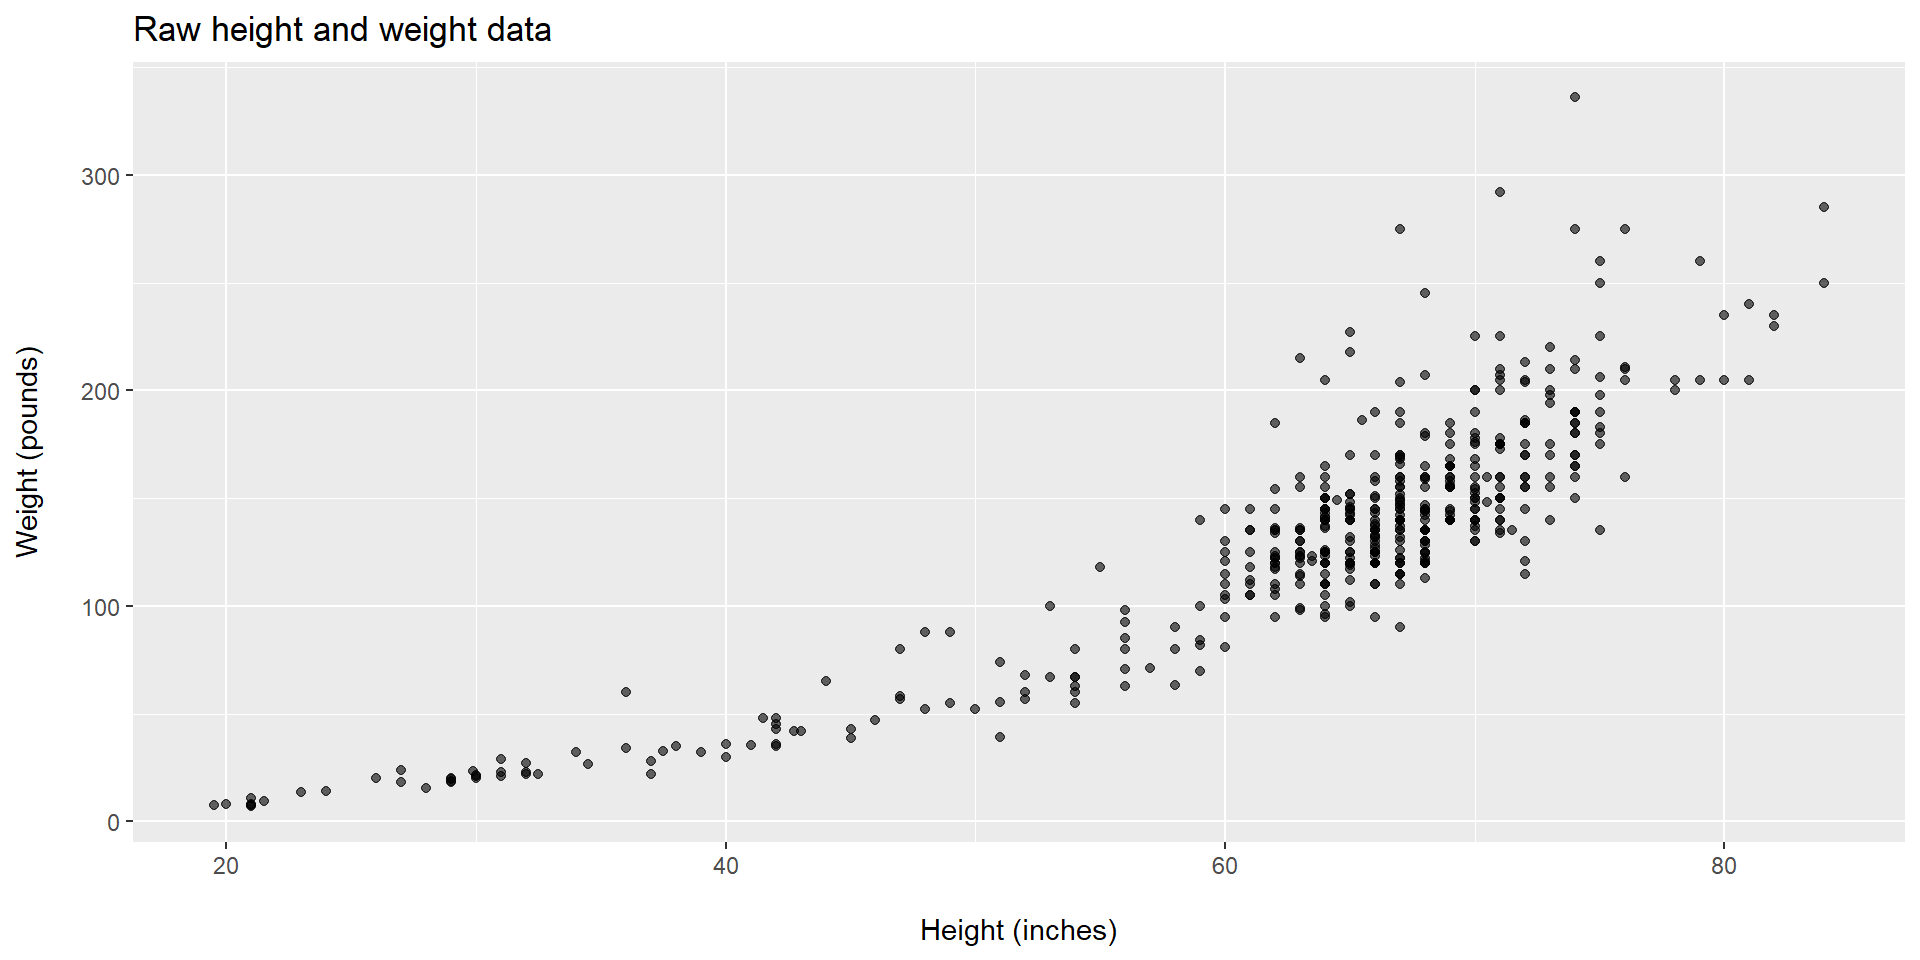
\includegraphics{C91ED_regression_interactions_files/figure-latex/unnamed-chunk-2-1.pdf}

\hypertarget{simulate-data-for-rural-group}{%
\paragraph{Simulate data for rural
group}\label{simulate-data-for-rural-group}}

\begin{itemize}
\tightlist
\item
  For this group, let's assume that their RT will be higher due to
  quieter living setting, with intercept 500ms and slope 3
\end{itemize}

\(Y_{i} = 500 + 3X_{i} + e_{i}\)

\begin{Shaded}
\begin{Highlighting}[]
\NormalTok{b0\_rural }\OtherTok{\textless{}{-}} \DecValTok{500}
\NormalTok{b1\_rural }\OtherTok{\textless{}{-}} \DecValTok{3}

\NormalTok{rural }\OtherTok{\textless{}{-}} \FunctionTok{tibble}\NormalTok{(}
  \AttributeTok{subj\_id =} \DecValTok{1}\SpecialCharTok{:}\NormalTok{n\_subj }\SpecialCharTok{+}\NormalTok{ n\_subj,}
  \AttributeTok{group =} \StringTok{"rural"}\NormalTok{,}
  \AttributeTok{b0 =}\NormalTok{ b0\_rural,}
  \AttributeTok{b1 =}\NormalTok{ b1\_rural,}
  \AttributeTok{dist\_level =} \FunctionTok{sample}\NormalTok{(}\DecValTok{0}\SpecialCharTok{:}\NormalTok{n\_subj, n\_subj, }\AttributeTok{replace =} \ConstantTok{TRUE}\NormalTok{),}
  \AttributeTok{err =} \FunctionTok{rnorm}\NormalTok{(n\_subj, }\AttributeTok{mean =} \DecValTok{0}\NormalTok{, }\AttributeTok{sd =} \DecValTok{80}\NormalTok{),}
  \AttributeTok{simple\_rt =}\NormalTok{ b0 }\SpecialCharTok{+}\NormalTok{ b1 }\SpecialCharTok{*}\NormalTok{ dist\_level }\SpecialCharTok{+}\NormalTok{ err)}
\end{Highlighting}
\end{Shaded}

\begin{itemize}
\tightlist
\item
  Now let's plot the data side by side
\end{itemize}

\begin{Shaded}
\begin{Highlighting}[]
\NormalTok{all\_data }\OtherTok{\textless{}{-}} 
  \FunctionTok{bind\_rows}\NormalTok{(urban, rural)}

\FunctionTok{ggplot}\NormalTok{(all\_data }\SpecialCharTok{\%\textgreater{}\%} \FunctionTok{mutate}\NormalTok{(}\AttributeTok{group =} \FunctionTok{fct\_relevel}\NormalTok{(group, }\StringTok{"urban"}\NormalTok{)), }
       \FunctionTok{aes}\NormalTok{(dist\_level, simple\_rt, }\AttributeTok{colour =}\NormalTok{ group)) }\SpecialCharTok{+}
  \FunctionTok{geom\_point}\NormalTok{() }\SpecialCharTok{+}
  \FunctionTok{geom\_smooth}\NormalTok{(}\AttributeTok{method =} \StringTok{"lm"}\NormalTok{, }\AttributeTok{se =} \ConstantTok{FALSE}\NormalTok{) }\SpecialCharTok{+}
  \FunctionTok{facet\_wrap}\NormalTok{(}\SpecialCharTok{\textasciitilde{}}\NormalTok{ group) }\SpecialCharTok{+} 
  \FunctionTok{theme}\NormalTok{(}\AttributeTok{legend.position =} \StringTok{"none"}\NormalTok{)}
\end{Highlighting}
\end{Shaded}

\begin{verbatim}
## `geom_smooth()` using formula = 'y ~ x'
\end{verbatim}

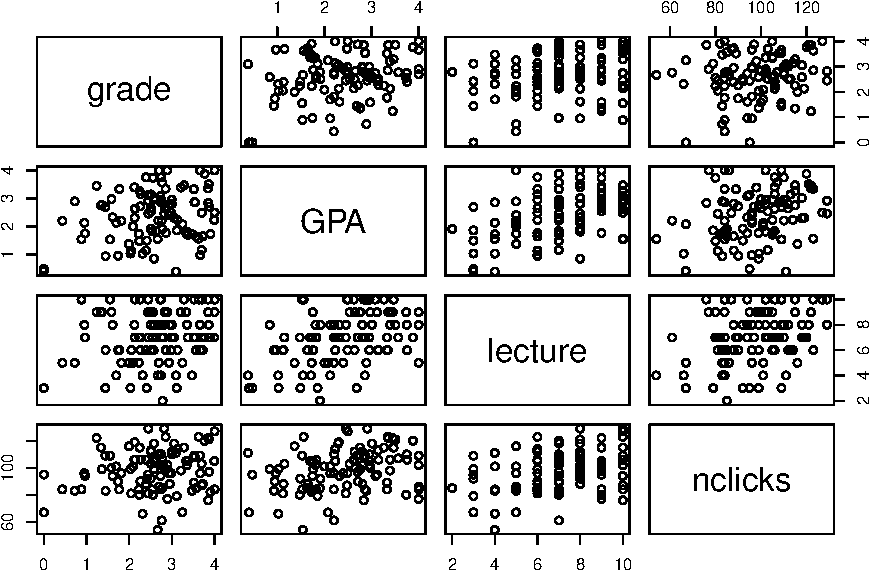
\includegraphics{C91ED_regression_interactions_files/figure-latex/unnamed-chunk-4-1.pdf}

\hypertarget{how-to-test-diference-between-slopes}{%
\subsubsection{How to test diference between
slopes}\label{how-to-test-diference-between-slopes}}

\begin{itemize}
\tightlist
\item
  Two separate regressions would not allow us to assess whether the two
  slopes significantly differ from one another.
\item
  We can represent one of the regression lines in terms of ``offset''
  values from the other

  \begin{itemize}
  \tightlist
  \item
    you can arbitrarily choose one group to represent the `baseline'
    (e.g., the ``urban'' group in the worked example in Chapter 4) and
    represent the y-intercept and slope of the other group as offsets
    from this baseline.
  \end{itemize}
\item
  So, if we treat the ``urban'' group as the baseline, we can express
  the y-intercept and slope for the ``rural'' groups in terms of two
  offsets \(\beta_{2}\) \& \(\beta_{3}\), for the y-intercept and slope,
  respectively.
\end{itemize}

y-intercept:
\(\beta_{0_\textit{_rural}} = \beta_{0_\textit{_urban}} + \beta_{2}\)

slope:
\(\beta_{1_\textit{_rural}} = \beta_{1_\textit{_urban}} + \beta_{3}\)

\begin{itemize}
\tightlist
\item
  The urban group had parameters \(\beta_{0_\textit{_urban}}\) = 450 and
  \(\beta_{1_\textit{_urban}}\) = 2, whereas the rural group had
  \(\beta_{0_\textit{_rural}}\) = 500 and \(\beta_{1_\textit{_urban}}\)
  = 3. Case in point:
\end{itemize}

\(\beta_{2}\) = 50, as \(\beta_{0_\textit{_rural}}\) -
\(\beta_{0_\textit{_urban}}\) = 500 - 450 = 50

\(\beta_{3}\) = 1, as \(\beta_{1_\textit{_rural}}\) -
\(\beta_{1_\textit{_urban}}\) = 3 - 2 = 1

\begin{itemize}
\tightlist
\item
  So, the two regression models become the following:
\end{itemize}

\(Y_{i_\textit{_urban}} = \beta_{0_\textit{_urban}} + \beta_{1_\textit{_urban}}X_{i} + e_{i}\)

and

\(Y_{i_\textit{_rural}} = (\beta_{0_\textit{_urban}} + \beta_{2}) + (\beta_{1_\textit{_urban}} + \beta_{3})X_{i} + e_{i}\)

\begin{itemize}
\tightlist
\item
  The final trick is to define an additional dummy predictor variable
  that takes on the value 0 for the urban group (chosen as our baseline)
  and 1 for the other group.
\end{itemize}

\hypertarget{final-interaction-model-with-dummy-coding}{%
\paragraph{Final interaction model with dummy
coding}\label{final-interaction-model-with-dummy-coding}}

\(Y_{i} = \beta_{0} + \beta_{1}X_{1i} + \beta_{2}X_{2i} + \beta_{3}X_{1i}X_{2i} + e_{i}\)

\begin{longtable}[]{@{}
  >{\raggedright\arraybackslash}p{(\columnwidth - 2\tabcolsep) * \real{0.3611}}
  >{\raggedright\arraybackslash}p{(\columnwidth - 2\tabcolsep) * \real{0.6389}}@{}}
\toprule\noalign{}
\begin{minipage}[b]{\linewidth}\raggedright
value
\end{minipage} & \begin{minipage}[b]{\linewidth}\raggedright
description
\end{minipage} \\
\midrule\noalign{}
\endhead
\bottomrule\noalign{}
\endlastfoot
\(X_{1i}\) & continuous predictor \\
\(X_{2i}\) & dummy coded variable taking on 0 for baseline and 1 for the
alternate group \\
\(\beta_{0}\) & y-intercept for the baseline group \\
\(\beta_{1}\) & slope for the baseline group \\
\(\beta_{2}\) & offset to y-intercept for the alternative group \\
\(\beta_{3}\) & offset to slope for the alternative group \\
\(\beta_{3}X_{1i}X_{2i}\) & interaction term \\
\end{longtable}

\hypertarget{code-you-own-categorical-predictors-in-factorial-designs}{%
\subsection{Code you own categorical predictors in factorial
designs}\label{code-you-own-categorical-predictors-in-factorial-designs}}

\begin{itemize}
\tightlist
\item
  default in R for categorical predictors are not ideal for experiments
\item
  default coding of categories gives you \textbf{simple effects} rather
  than \textbf{main effects} (typically, you'll want the latter)
\item
  coding categorical predictors by hand is best practice
\item
  don't include them as factor variables either - R isn't very good at
  handling these
\end{itemize}

\hypertarget{coding-scheme-for-categorical-variables}{%
\subsubsection{Coding scheme for categorical
variables}\label{coding-scheme-for-categorical-variables}}

\hypertarget{simple-effects-vs-main-effects}{%
\paragraph{Simple effects vs main
effects}\label{simple-effects-vs-main-effects}}

\begin{itemize}
\tightlist
\item
  In an \(A \times B\) design, the \emph{simple effect of \(A\)} is the
  effect of \(A\) controlling for \(B\)
\item
  Whilst the \emph{main effect of \(A\)} is the effect of \(A\)
  \textbf{ignoring} \(B\)
\item
  The distinction between simple interactions and main interactions has
  the same logic: the simple interaction of \(AB\) in an \(ABC\) design
  is the interaction of \(AB\) at a particular level of \(C\); the main
  interaction of \(AB\) is the interaction \textbf{ignoring} \(C\).
\item
  The latter is what we are usually talking about when we talk about
  lower-order interactions in a three-way design. It is also what is
  generated in the standard ANOVA output in R using the \texttt{aov}
  function.
\end{itemize}

\hypertarget{the-key-coding-schemes}{%
\paragraph{The key coding schemes}\label{the-key-coding-schemes}}

\begin{itemize}
\tightlist
\item
  You're coding scheme will impact

  \begin{itemize}
  \tightlist
  \item
    the intercept term in the model
  \item
    the interpretation of the tests for all but the highest-order
    effects and interaction in factorial design
  \end{itemize}
\item
  It can also influence the interpretation/estimation of random effects
  in a mixed-effects model
\item
  If you have a design with only a single two-level factor, and are
  using maximal random-effects structure, the choice of coding scheme
  doesn't really matter.
\end{itemize}

For a two-level factor, you could use the following codes

\begin{longtable}[]{@{}lll@{}}
\toprule\noalign{}
Scheme & \(A_{1}\) & \(A_{2}\) \\
\midrule\noalign{}
\endhead
\bottomrule\noalign{}
\endlastfoot
Treatment (dummy) & 0 & 1 \\
Sum & -1 & 1 \\
Deviation & \(-\frac{1}{2}\) & \(\frac{1}{2}\) \\
\end{longtable}

\hypertarget{what-about-factors-with-more-than-two-levels}{%
\paragraph{What about factors with more than two
levels?}\label{what-about-factors-with-more-than-two-levels}}

\begin{itemize}
\tightlist
\item
  A factor with \(k\) levels requires \(k-1\) variables
\item
  Each predictor contrasts a particular ``target'' level of the factor
  with a level that you (arbitrarily) choose as the ``baseline'' level
\item
  For example, a three level factor \(A\) with \(A1\) chosen as the
  baseline would include two predictors, comparing \(A2\) and \(A1\) and
  the other comparing \(A3\) to \(A1\).
\item
  For treatment coding, the target level is set to 1, otherwise 0.
\item
  For sum coding, the levels must sum to zero, so for a given predictor,
  the target level is given the value 1, the baseline is given the value
  -1, and any other level is given the value 0
\item
  For deviation coding, the values must also sum to 0. Deviation coding
  is recommended whenever you are trying to draw ANOVA-style inferences.
  Un this scheme, the target level gets the value \(\frac{k-1}{k}\)
  while any non-target level get the value \(-\frac{1}{k}\)
\end{itemize}

\textbf{Three level factor example}

\emph{Treatment (Dummy)}

\begin{longtable}[]{@{}lll@{}}
\toprule\noalign{}
Level & A2v1 & A3v1 \\
\midrule\noalign{}
\endhead
\bottomrule\noalign{}
\endlastfoot
A1 & 0 & 0 \\
A2 & 1 & 0 \\
A3 & 0 & 1 \\
\end{longtable}

\emph{Sum}

\begin{longtable}[]{@{}lll@{}}
\toprule\noalign{}
Level & A2v1 & A3v1 \\
\midrule\noalign{}
\endhead
\bottomrule\noalign{}
\endlastfoot
A1 & -1 & -1 \\
A2 & 1 & 0 \\
A3 & 0 & 1 \\
\end{longtable}

\emph{Deviation}

\begin{longtable}[]{@{}lll@{}}
\toprule\noalign{}
Level & A2v1 & A3v1 \\
\midrule\noalign{}
\endhead
\bottomrule\noalign{}
\endlastfoot
A1 & \(-\frac{1}{3}\) & \(-\frac{1}{3}\) \\
A2 & \(\frac{2}{3}\) & \(-\frac{1}{3}\) \\
A3 & \(-\frac{1}{3}\) & \(\frac{2}{3}\) \\
\end{longtable}

\hypertarget{how-to-create-your-own-numeric-predictors}{%
\subsubsection{How to create your own numeric
predictors}\label{how-to-create-your-own-numeric-predictors}}

\begin{Shaded}
\begin{Highlighting}[]
\DocumentationTok{\#\# create your own numeric predictors}
\DocumentationTok{\#\# make an example table}
\NormalTok{dat }\OtherTok{\textless{}{-}} \FunctionTok{tibble}\NormalTok{(}\AttributeTok{Y =} \FunctionTok{rnorm}\NormalTok{(}\DecValTok{12}\NormalTok{),}
             \AttributeTok{A =} \FunctionTok{rep}\NormalTok{(}\FunctionTok{paste0}\NormalTok{(}\StringTok{"A"}\NormalTok{, }\DecValTok{1}\SpecialCharTok{:}\DecValTok{3}\NormalTok{), }\AttributeTok{each =} \DecValTok{4}\NormalTok{))}
\end{Highlighting}
\end{Shaded}

Treatment coding

\begin{Shaded}
\begin{Highlighting}[]
\DocumentationTok{\#\# examples of three level factors}
\DocumentationTok{\#\# treatment coding}
\NormalTok{dat\_treat }\OtherTok{\textless{}{-}}\NormalTok{ dat }\SpecialCharTok{\%\textgreater{}\%}
  \FunctionTok{mutate}\NormalTok{(}\AttributeTok{A2v1 =} \FunctionTok{if\_else}\NormalTok{(A }\SpecialCharTok{==} \StringTok{"A2"}\NormalTok{, 1L, 0L),}
     \AttributeTok{A3v1 =} \FunctionTok{if\_else}\NormalTok{(A }\SpecialCharTok{==} \StringTok{"A3"}\NormalTok{, 1L, 0L))}

\NormalTok{dat\_treat}
\end{Highlighting}
\end{Shaded}

\begin{verbatim}
## # A tibble: 12 x 4
##         Y A      A2v1  A3v1
##     <dbl> <chr> <int> <int>
##  1  0.408 A1        0     0
##  2  0.630 A1        0     0
##  3 -0.676 A1        0     0
##  4 -0.891 A1        0     0
##  5 -0.410 A2        1     0
##  6 -1.44  A2        1     0
##  7 -2.01  A2        1     0
##  8  0.562 A2        1     0
##  9 -0.671 A3        0     1
## 10  1.00  A3        0     1
## 11 -1.61  A3        0     1
## 12  0.322 A3        0     1
\end{verbatim}

Sum coding

\begin{Shaded}
\begin{Highlighting}[]
\DocumentationTok{\#\# sum coding}
\NormalTok{dat\_sum }\OtherTok{\textless{}{-}}\NormalTok{ dat }\SpecialCharTok{\%\textgreater{}\%}
  \FunctionTok{mutate}\NormalTok{(}\AttributeTok{A2v1 =} \FunctionTok{case\_when}\NormalTok{(A }\SpecialCharTok{==} \StringTok{"A1"} \SpecialCharTok{\textasciitilde{}} \SpecialCharTok{{-}}\NormalTok{1L, }\CommentTok{\# baseline}
\NormalTok{                          A }\SpecialCharTok{==} \StringTok{"A2"} \SpecialCharTok{\textasciitilde{}}\NormalTok{ 1L,  }\CommentTok{\# target}
                          \ConstantTok{TRUE}      \SpecialCharTok{\textasciitilde{}}\NormalTok{ 0L), }\CommentTok{\# anything else}
         \AttributeTok{A3v1 =} \FunctionTok{case\_when}\NormalTok{(A }\SpecialCharTok{==} \StringTok{"A1"} \SpecialCharTok{\textasciitilde{}} \SpecialCharTok{{-}}\NormalTok{1L, }\CommentTok{\# baseline}
\NormalTok{                          A }\SpecialCharTok{==} \StringTok{"A3"} \SpecialCharTok{\textasciitilde{}}\NormalTok{  1L, }\CommentTok{\# target}
                          \ConstantTok{TRUE}      \SpecialCharTok{\textasciitilde{}}\NormalTok{ 0L)) }\CommentTok{\# anything else}

\NormalTok{dat\_sum}
\end{Highlighting}
\end{Shaded}

\begin{verbatim}
## # A tibble: 12 x 4
##         Y A      A2v1  A3v1
##     <dbl> <chr> <int> <int>
##  1  0.408 A1       -1    -1
##  2  0.630 A1       -1    -1
##  3 -0.676 A1       -1    -1
##  4 -0.891 A1       -1    -1
##  5 -0.410 A2        1     0
##  6 -1.44  A2        1     0
##  7 -2.01  A2        1     0
##  8  0.562 A2        1     0
##  9 -0.671 A3        0     1
## 10  1.00  A3        0     1
## 11 -1.61  A3        0     1
## 12  0.322 A3        0     1
\end{verbatim}

Deviation coding

\begin{Shaded}
\begin{Highlighting}[]
\DocumentationTok{\#\# deviation coding}
\DocumentationTok{\#\# baseline A1}
\NormalTok{dat\_dev }\OtherTok{\textless{}{-}}\NormalTok{ dat }\SpecialCharTok{\%\textgreater{}\%}
  \FunctionTok{mutate}\NormalTok{(}\AttributeTok{A2v1 =} \FunctionTok{if\_else}\NormalTok{(A }\SpecialCharTok{==} \StringTok{"A2"}\NormalTok{, }\DecValTok{2}\SpecialCharTok{/}\DecValTok{3}\NormalTok{, }\SpecialCharTok{{-}}\DecValTok{1}\SpecialCharTok{/}\DecValTok{3}\NormalTok{), }\CommentTok{\# target A2}
         \AttributeTok{A3v1 =} \FunctionTok{if\_else}\NormalTok{(A }\SpecialCharTok{==} \StringTok{"A3"}\NormalTok{, }\DecValTok{2}\SpecialCharTok{/}\DecValTok{3}\NormalTok{, }\SpecialCharTok{{-}}\DecValTok{1}\SpecialCharTok{/}\DecValTok{3}\NormalTok{)) }\CommentTok{\# target A3}

\NormalTok{dat\_dev}
\end{Highlighting}
\end{Shaded}

\begin{verbatim}
## # A tibble: 12 x 4
##         Y A       A2v1   A3v1
##     <dbl> <chr>  <dbl>  <dbl>
##  1  0.408 A1    -0.333 -0.333
##  2  0.630 A1    -0.333 -0.333
##  3 -0.676 A1    -0.333 -0.333
##  4 -0.891 A1    -0.333 -0.333
##  5 -0.410 A2     0.667 -0.333
##  6 -1.44  A2     0.667 -0.333
##  7 -2.01  A2     0.667 -0.333
##  8  0.562 A2     0.667 -0.333
##  9 -0.671 A3    -0.333  0.667
## 10  1.00  A3    -0.333  0.667
## 11 -1.61  A3    -0.333  0.667
## 12  0.322 A3    -0.333  0.667
\end{verbatim}

\hypertarget{interactions-conclusions}{%
\subsection{Interactions: conclusions}\label{interactions-conclusions}}

\begin{itemize}
\tightlist
\item
  The interpretation of all but the highest order effect depends on the
  coding scheme
\item
  The treatment coding, you are looking at simple effects and simple
  interactions, \textbf{not} main effects and main interactions
\item
  The parameter estimates for sum coding differs from deviation coding
  only in the magnitude of the parameter estimates, but have identical
  interpretations.
\item
  Because it is not subject to scaling effects seen under sum coding,
  deviation should be used by default for ANOVA-style designs
\item
  The default coding for factors in R is ``treatment'' coding
\item
  To obtain canonical ANOVA-style interpretations of main effects and
  interactions use \textbf{deviation coding NOT the default treatment
  coding}.
\end{itemize}

\end{document}
